\documentclass[10pt,twocolumn, a4j]{jsarticle}


\usepackage[dvipdfmx]{graphicx}
\usepackage{amsmath}
\usepackage{eepic}

\setlength{\oddsidemargin}{-12mm}
\setlength{\topmargin}{-16mm}
\setlength{\textwidth}{181mm}
\setlength{\columnsep}{8mm}

%下端マージン,行間を調整するには、下記のパラメータを調整する
\setlength{\textheight}{248mm}
\renewcommand{\baselinestretch}{.856}

\pagestyle{empty}


\makeatletter
\def\@biblabel#1{#1)}
\def\@cite#1{#1)}
\makeatother

\begin{document}


\twocolumn[

{\LARGE
\hspace*{17mm}55\hspace*{12mm}
Bitcoin のトランザクションにおける
}


{\LARGE
\hspace*{28mm}\hspace*{12mm}
Segwit と Taproot に関する分析
}


\vspace{-2mm}
\begin{flushright}
電子商取引研究室\hspace{1.5zw}阪本 翔\hspace{1.5zw}
\end{flushright}
\vspace{3mm}
]

\renewcommand{\thesection}{\arabic{section} .}

%以下の7行はタイトルの左端からの距離が,指示通になっているかどうかを
%示す矢印の出力です.
%レジメ作成の際には削除又はコメントアウトしてください.

%ここから
\unitlength = 1mm
\begin{picture}(50,10)
% \put(23,20){\vector(1,0){10}}
% \put(13,19){\scriptsize 36mm}
% \put(10,20){\vector(-1,0){10}}
\end{picture}
\vspace{-1.2cm}
%ここまで



\section{序 論}

Satoshi Nakamotoが2008年にビットコインを発表して以来、現在も暗号資産全体の約39%をビットコインが占めている。しかし、ビットコインには「スケーラビリティ問題」と「トランザクション展性」と呼ばれる問題がある。これに対し2017年8月にSegwitと呼ばれるビットコインプロトコルの拡張が行われ現在でもこの問題の改善に役立っている。また2021年11月にTaprootと呼ばれるSegwitをアップデートした形のビットコインプロトコルの拡張が行われ現在も実装されており今後のビットコインの脆弱な上記のような問題をカバーするものになると考えられている。そこでSegwitとTaprootに関する使用率を正確に調査することでビットコインに対する利便性がどの程度あるのかを調査し評価する。


\section{ビットコイン問題}
ビットコインにはデータ容量制限が原因の「スケーラビリティ問題」と外部からトランザクションIDによって改ざんが可能である「トランザクション展性」と呼ばれる問題があり、この問題に対しトランザクションを圧縮してデータ量を小さくする(署名データを分離してブロックに保存する)技術であるSegwitが2017年8月に導入された。その後Segwitのアップデート版となるTaprootはMASTとシュノア署名と呼ばれる技術を融合し、さらなるスケーラビリティの向上とプライバシー機能の改善が実現される。

\section{トランザクション情報検索システム}
SegwitとTaprootの使用率を調査するにあたり、ビットコインを送金する際に生じるトランザクション(取引履歴)の情報を取得するためにブロックチェーンのAPIを用いて765,263個(2022年11月30日時点)のビットコインブロックをダウンロードしブロック情報を全てデータベースに格納する。その後、データベースに格納したブロックのトランザクションに対しSegwitとTaprootを識別するために必要なビットコインを送金するために用いられるアドレス(=addr)を検索するシステムを作成し、システムを通して得たSegwitとTaprootが該当するアドレスの数をトランザクションのアドレスの全数で割ったものをSegwitとTaprootの使用率としグラフ化する。

\section{結果・考察}
図\ref{fig:segwit}のグラフより導入開始されたSegwitは2019年の600,000ブロックで約5割の使用率となっており、2022年時点では約8割の使用率となっているため増加傾向にあるとわかる。
図\ref{fig:taproot}のグラフよりTaprootはまだ1年間のみの実装と期間が短いため十分なデータが取れなく、ビットコインに対し有用的であるかどうかが判別しずらくなっている。しかしTaprootはこれまでビットコインに実装されることのなかった「スマートコンストラクト」の機能の拡張が実現されることが予想されており、近年アルトコインで普及しているNFTがビットコインで普及すると考えられ多くのユースケースが実装されると予想される。

\begin{figure}[h]
    \centering
    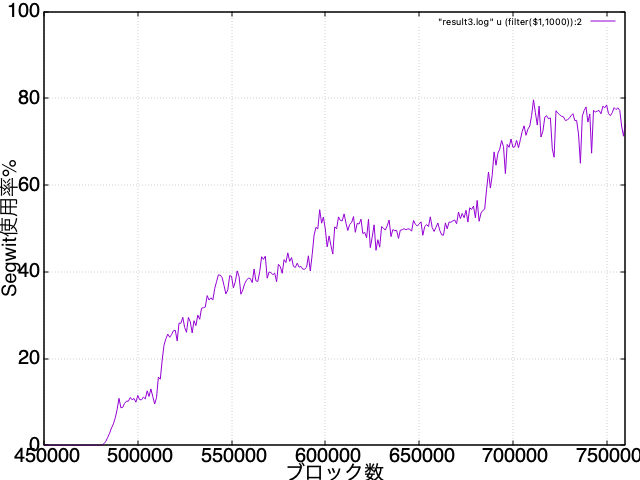
\includegraphics[width=0.3\textwidth]{segwitfigure.png}
    \caption{Segwitの使用率}
    \label{fig:segwit}
\end{figure}

\begin{figure}[h]
    \centering
    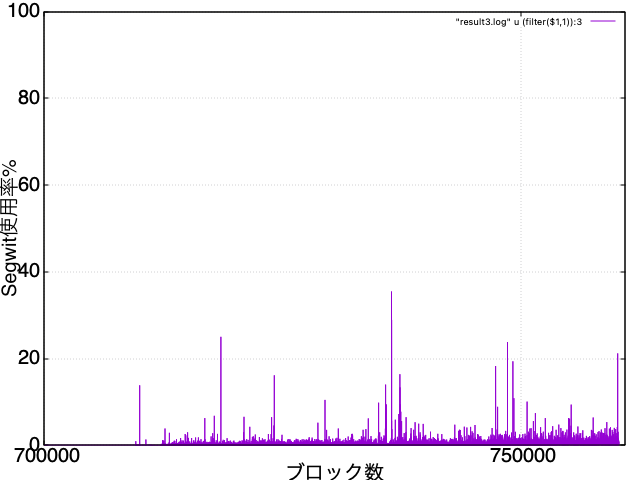
\includegraphics[width=0.3\textwidth]{taprootfigure.png}
    \caption{Taprootの使用率}
    \label{fig:taproot}
\end{figure}



\section{結論}
ビットコインの問題に対した改善案として挙げられるSegwitとTaprootの使用率を求める検索システムを提案し、ビットコインにおけるSegwitとTaprootの使用率をグラフで可視化することで重要性が理解できた。また、Taprootのように未だ使用率がよくないのは実装期間が浅いためであり、Segwitと同様に先の5年〜10年のデータをもとにグラフ化することでTaprootの有用性がわかると考える。

%本来は\cite{kinosita}等として、本文中で引用された文献のみリストに
%掲載されます。\nociteは本文で引用されていない文献をリストに加える
%命令なので、実際に予稿を作成する際には使用してはいけません。


\makeatletter
\def\@biblabel#1{#1)}
\makeatother

%下記は半自動で文献リストを生成する方法です。
%できれば、全自動で文献リストを生成するbibTeXを
%使用してください。

%bibTeXを使う場合は、ここから

\begin{thebibliography}{1}

\bibitem{}
  Satoshi Nakamoto. Bitcoin: A peer-to-peer electronic cash system. https://bitcoin.org, 2008.

\end{thebibliography}
%ここまでをコメントアウトして以下の\bibliographyの行のコメントアウトを解除し、
%pbibtexコマンドを実行してください。

%\bibliography{reference}

\bibliographystyle{tipsj}   


\end{document}
